% !TEX program = xelatex
\documentclass[]{article}
\usepackage{commons/course}

\begin{document}
\printheader

\section{}
\section{}
\subsection{}
برای ساخت کلید من از
\link{https://irtfweb.ifa.hawaii.edu/~lockhart/gpg/}{این}
لینک استفاده کردم. همان طور که مشخص است در ابتدا از دستور
\LRE{\verb|gpg --gen-key|}
استفاده می‌کنیم. در ادامه تمامی موارد خواسته شده را وارد می‌کنیم و یک پسورد برای کلید خود انتخاب می‌کنیم.
نتیجه دستور در شکل
\ref{fig:gpg:keygen}
موجود است.
\begin{figure}[H]
    \centering
    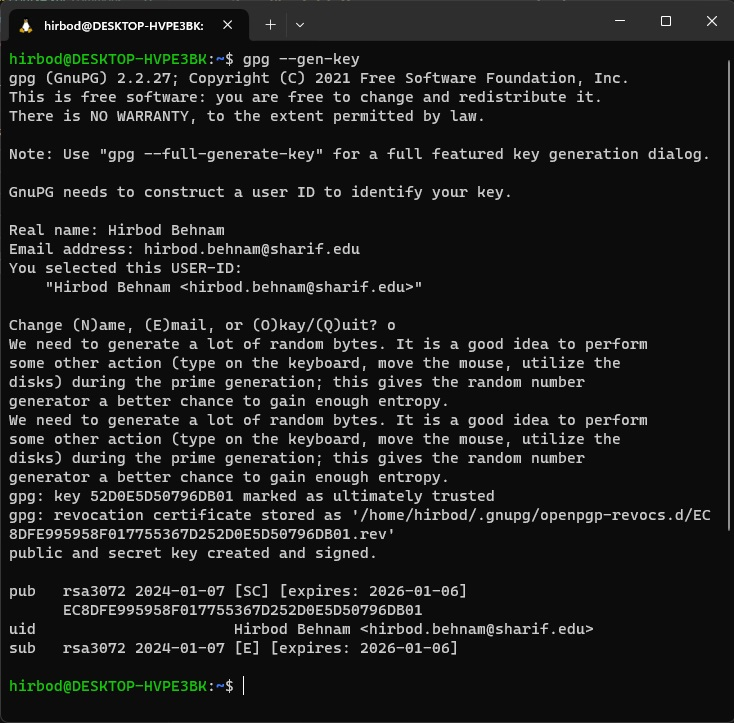
\includegraphics[scale=0.5]{pics/gpg-keygen.jpg}
    \caption{ساخت \lr{GPG key}}
    \label{fig:gpg:keygen}
\end{figure}
حال می‌توانیم با دستور
\LRE{\verb|gpg --list|}
تمامی کلید‌های خود را مشاهده کنیم. همچنین می‌توان با دستور زیر کلید عمومی مربوط به دانشگاه را استخراج کرد.
\begin{latin}
\begin{lstlisting}[language=sh]
gpg --export -a "hirbod.behnam@sharif.edu"
\end{lstlisting}
\end{latin}
نتیجه این دستورات را می‌توانید در شکل
\ref{fig:gpg:view}
ببینید.
\begin{figure}[H]
    \centering
    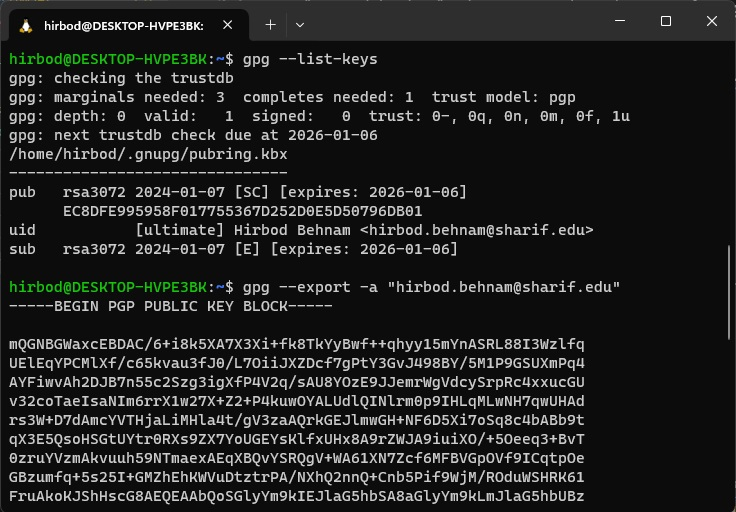
\includegraphics[scale=0.5]{pics/gpg-view.jpg}
    \caption{مشاهده کلید‌های PGP}
    \label{fig:gpg:view}
\end{figure}
\subsection{}
در این قسمت در ابتدا نیاز است که کلید عمومی داده شده را
import
کنیم. برای این کار از دستور زیر استفاده می‌کنیم. نتیجه‌ی آن در عکس
\ref{fig:gpg:import}
آمده است.
\begin{latin}
\begin{lstlisting}[language=sh]
gpg --import Reza_0xCFBEEE88_public.asc
\end{lstlisting}
\end{latin}
\begin{figure}[H]
    \centering
    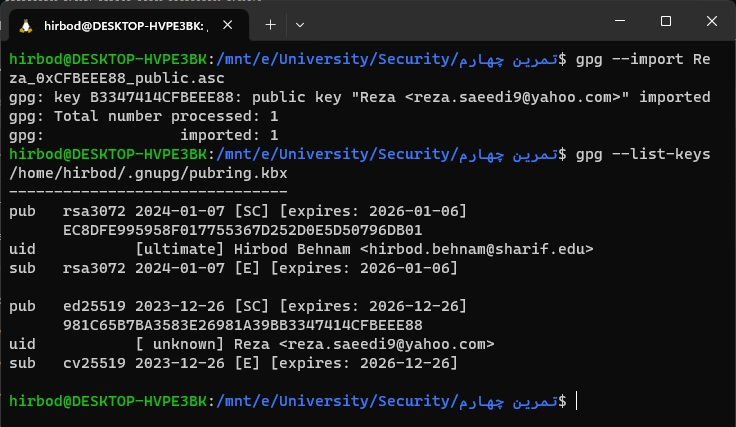
\includegraphics[scale=0.5]{pics/gpg-import.jpg}
    \caption{اضافه کردن کلید PGP طراح تمرین به GPG}
    \label{fig:gpg:import}
\end{figure}
حال باید دیتایی را در ابتدا امضا و سپس رمزنگاری کنیم. برای این کار از دستور زیر استفاده می‌کنیم.
دقت کنید که این دستور یک فایل را رمزنگاری و امضا می‌کند. در نتیجه کافی است که صرفا متن ایمیل را در فایلی
بنویسیم و آن فایل را رمز کنیم.
(\link{https://medium.com/@acparas/how-to-encrypt-and-sign-a-file-with-gpg-531070b2fa6d}{منبع})
\begin{latin}
\begin{lstlisting}[language=sh]
    gpg --output email.pgp --armor --encrypt --sign --recipient reza.saeedi9@yahoo.com email-plaintext.txt
\end{lstlisting}
\end{latin}
همان طور که مشاهده می‌کنید محتوای فایل تولید شده رمزگذاری شده است.
\begin{figure}[H]
    \centering
    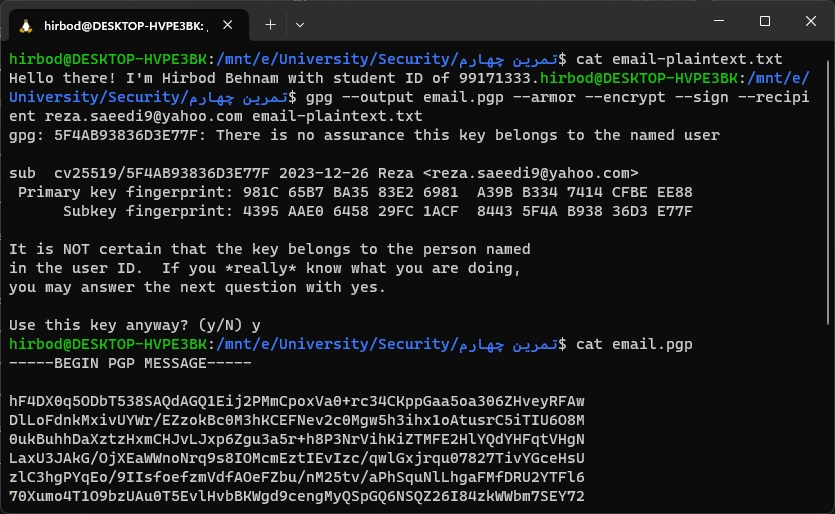
\includegraphics[scale=0.5]{pics/gpg-encrypt.jpg}
    \caption{رمزنگاری پیام}
    \label{fig:gpg:encrypt}
\end{figure}
در نهایت نیز محتوای این فایل را ایمیل کردم. دقت کنید که در کل مراحل بالا
\verb|--armor|
برای این بود که نتیجه به صورت اسکی کد باشد و بتوان آن را کپی و پیست در ایمیل کرد.
ایمیل فرستاده شده نیز در شکل
\ref{fig:gpg:email}
قابل مشاهده است.
\begin{figure}[H]
    \centering
    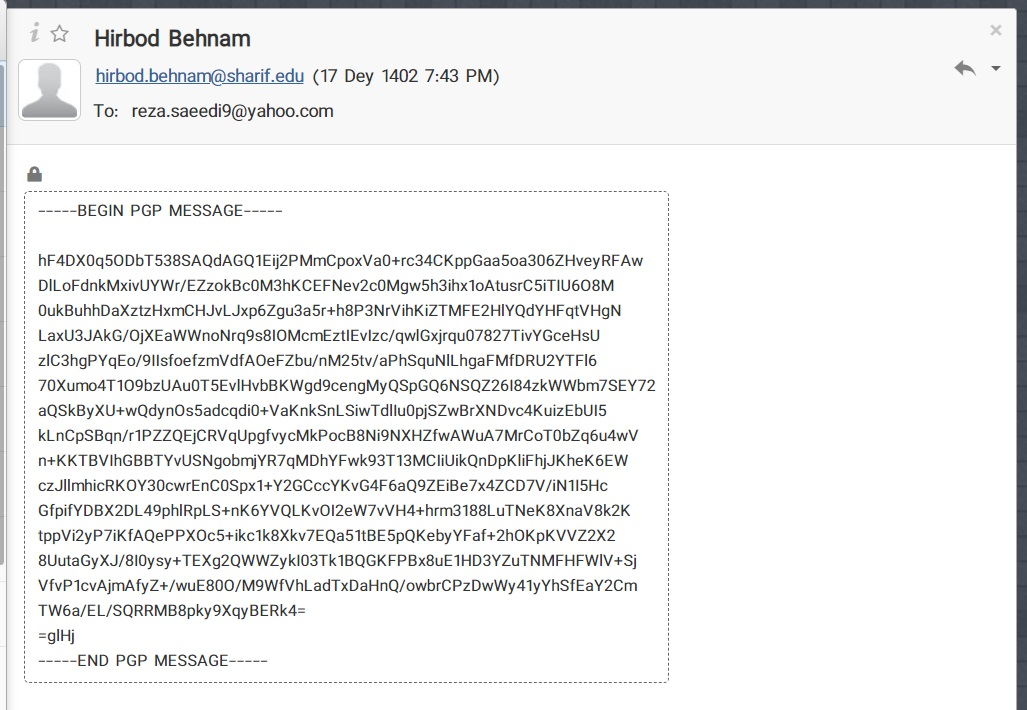
\includegraphics[scale=0.35]{pics/gpg-email.jpg}
    \caption{ایمیل فرستاده شده}
    \label{fig:gpg:email}
\end{figure}
\section{}
\section{}
\section{}
\end{document}
